\documentclass[conf]{new-aiaa}
%\documentclass[journal]{new-aiaa} for journal papers
\usepackage[utf8]{inputenc}

\usepackage{graphicx}
\usepackage{amsmath}
\usepackage[version=4]{mhchem}
\usepackage{siunitx}
\usepackage{longtable,tabularx}
\setlength\LTleft{0pt} 

\title{Model-Based CubeSat Flight-Software Architecture using a Docs-as-Code approach}

\author{First A. Author\footnote{Insert Job Title, Department Name, Address/Mail Stop, and AIAA Member Grade (if any) for first author.} and Second B. Author Jr.\footnote{Insert Job Title, Department Name, Address/Mail Stop, and AIAA Member Grade (if any) for second author.}}
\affil{Business or Academic Affiliation 1, City, State, Zip Code}
\author{Third C. Author\footnote{Insert Job Title, Department Name, Address/Mail Stop, and AIAA Member Grade (if any) for third author.}}
\affil{Business or Academic Affiliation 2, City, Province, Zip Code, Country}
\author{Fourth D. Author\footnote{Insert Job Title, Department Name, Address/Mail Stop, and AIAA Member Grade (if any) for fourth author (etc.).}}
\affil{Business or Academic Affiliation 2, City, State, Zip Code}

\begin{document}

\maketitle

\begin{abstract}
PLACEHOLDER
\end{abstract}

\section{Nomenclature}

{\renewcommand\arraystretch{1.0}
\noindent\begin{longtable*}{@{}l @{\quad=\quad} l@{}}
$A$  & amplitude of oscillation \\
$a$ &    cylinder diameter \\
$C_p$& pressure coefficient \\
$Cx$ & force coefficient in the \textit{x} direction \\
$Cy$ & force coefficient in the \textit{y} direction \\
c   & chord \\
d$t$ & time step \\
$Fx$ & $X$ component of the resultant pressure force acting on the vehicle \\
$Fy$ & $Y$ component of the resultant pressure force acting on the vehicle \\
$f, g$   & generic functions \\
$h$  & height \\
$i$  & time index during navigation \\
$j$  & waypoint index \\
$K$  & trailing-edge (TE) nondimensional angular deflection rate
\end{longtable*}}

\section{Introduction}
\lettrine{T}{his} article presents the Mach30 modeling language (m30ml), tools, and technical approach used to facilitate the configuration management, design, specification, & implementation of the SeaLion mission architecture for the flight software.

The m30ml was created based on a model-based systems engineering (MBSE) approach to systems engineering whereby models, as opposed to documents, serve as the authoritative source of truth for conducting systems engineering activities, such as the design, specification, analysis, verification & validation of a system \cite:{architecting_spacecraft}.

For the SeaLion Mission, a joint CubeSat mission between the Old Dominion University and Coast Guard Academy, the flight software team adopted an MBSE approach to flight software architecture, using a docs-as-code approach \cite:{docs_as_code}, whereby the same tools and methodologies for managing software are also used for configuration management of documentation. Applying both an MBSE and docs-as-code approach means that aspects of the mission architecture, such as stakeholder needs, user stories, and data structures pertaining to the CubeSat mission, are captured are within a model that is both human-readable and machine-queryable.

\section{SeaLion Mission}

The SeaLion mission is a collaborative mission between Old Dominion University (ODU), the United Stated Coast Guard Academy (USCGA), and the Air Force Institute of Technology (AFIT) to design and produce a 3-Unit (3U) CubeSat.

SeaLion consists of three payloads for on-orbit validation.  ODU provided one payload while the USCGA and AFIT provided the other two payloads.  SeaLion is planned to fly as a secondary payload on a Northrop Grumman Antares Rocket from Wallops Flight Facility (WFF), currently scheduled for March, 2023 \cite:{sealion_cdr}.

\section{CubeSats}

The CubeSat, originating from California Polytechnic State University in 1999, are a standardized form of nanosatellites.  Nanosatellites are satellites typically defined with a mass of less than 10 kg.  CubeSats, also known as Cube Satellites, are defined by standardized and modular architecture of 1-Unit (1U) cubes with dimensions of 10 cm X 10 cm X 10 cm with a maximum mass of 1.33 kg \cite:{cubesat_standard}.  These units can be stacked such as, for example, a 3U CubeSat with standard dimensions of 10 cm X 10 cm X 34.05 cm +/- 0.03 cm and a maximum mass of 4.00 kg \cite:{cubesat_standard}.

\subsection{CubeSat Users}

CubeSats were initially conceived as educational tools for space systems engineering \cite:{heidt_new}.  Now, their roles have been expanded to not only just educational tools but for observation, technology demonstrations, and research that were previous monopolized by much larger satellites due to the aforementioned low cost of production and launch of these satellites.  As such, there has been increasing popularity for CubeSats ass seen by the number of launches in \ref{swartwout_data_graph} since year 2000 \cite:{swartwout_data}.

University groups especially are a large contributor in the overall number of launches of CubeSats yearly with university groups consistently maintaining plurality on total launches \cite:{swartwout_data}. Thus, a need for readily available and easily learnable tools for students especially exists for those who are new to both CubeSat design and systems engineering.

\begin{figure}[hbt!]
    \centering
    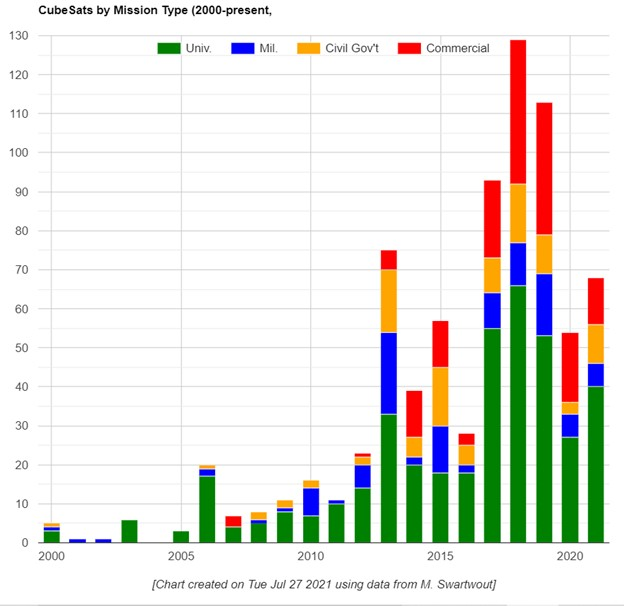
\includegraphics[width=.5\textwidth]{swartwout_data_graph}
    \caption{Nanosatellite launch data provided by M. Swartwout \cite:{swartwout_data}.}
    \label{swartwout_data_graph}
\end{figure}

\section{Goals}

The goal of the SeaLion CubeSat flight software architecture was to capture the data structures and expected behaviors of the flight software, such that it can be unambiguiously understood enough to be implemented, as well as provide full traceability and rationale for architectural elements with minimal configuration management overhead \cite:{sealion_mission_architecture}.

The MBSE approach was of interest to the SeaLion CubeSat flight software team, as to yield the benefits of reducing ambiguity that usually comes with using informal language for specifying aspects of a system, as well as minimizing duplication of content that tends to accumulate in a document-based systems engineering approach.

Selection of a modeling language, modeling tool, and technical approach needs to be taken into consideration, in order to properly adopt a MBSE approach.  The m30ml MBSE approach uses the Docs as Code and the Ontological Modeling Language (OML) as its basis of design.

Other considerations include overhead incurred with training the team, as well as technical overhead with setting up and maintaining the modeling tools.

\subsection{Model-Based Systems Engineering}

Traditional approaches use documents as their authoritative source of truth for conducting system engineering activities \cite:{architecting_spacecraft}.  However, these documents often do not have a living relationship with other documents or to other corresponding elements; thus, changes to one document require manual changes to other documents \cite:{ibm_mbse}.  Models provide the following key advantages over document-based approaches \cite:{ibm_mbse}:

\begin{enumerate}
\item Information is readily communicated and shared within the project \cite:{ibm_mbse}.

\item Changes are easily accommodated \cite:{ibm_mbse}.

\item Traceability is automated \cite:{ibm_mbse}.

\item PLACEHOLDER
\end{enumerate}

The m30ml MBSE approach uses the Docs as Code and the Ontological Modeling Language (OML) as its basis of design.

\subsection{Docs As Code Approach}

Documentation as Code, or also known as Docs as Code, refers to a philosophy that you should be writing documentation with the same tools as code \cite:{docs_as_code}.  These tools may include version control (e.g., Git), issue trackers, code tools, etc.

\begin{quoting}
    This means following the same workflows as development teams, and being integrated in the product team. It enables a culture where writers and developers both feel ownership of documentation, and work together to make it as good as possible \cite:{docs_as_code}. 
\end{quoting}

It was of interest to adopt a docs-as-code approach, as to yield the benefits of utilizing the same tools used to manage code, using version control tools (e.g., Git), for the configuration management of flight software architecture documentation, captured in a model-based approach \cite:{docs_as_code}.

\subsection{Ontological Modeling Language}

PLACEHOLDER

\section{Mach30 Modelling Language}

The SeaLion Architecture uses m30ml to specify references, stakeholder needs, user stories, & data structures for facilitating traceability of design decisions within the Mission ConOps \cite:{mach30_git}.  The SeaLion repository is also structured as a Distributed OSHW Framework (DOF)-component for defining the contents of the Mission ConOps as a collection of nested subcomponents, component interfaces, and component functions for generating bill of materials (BOMs), assembly instructions, and/or usage documentation.

This is all done in an effort to execute the project via a documentation as code philosophy. A philosophy in which documentation is written with the same tools as code \cite:{docs_as_code}. This allows for workflows between development teams to be more closely integrated.

\subsection{Modeling Language, Tool, & Methodology}

The Mach30 modeling language (m30ml) is a YAML-based modeling language for defining a software architecture. Since YAML is a lightweight, highly-structured, human-readable, machine queryable, and line-oriented markup language, it was ideal for document generation use cases, as well as use with version control tools like Git.

Mach30 also had minimal technical overhead as it was compatible with modern doc tools such as asciidoctor & bibtex.

Mach30 also provided modeling elements familiar in agile software development, such as stakeholder needs, user stories, and data structures, with relationship elements for defining traceability between modeling elements.

For the aforementioned reasons, the SeaLion CubeSat flight software team downselected m30ml for specifying the SeaLion CubeSat flight software architecture \cite:{mach30_git}.

\subsection{Stakeholder Needs}

The SeaLion project's methodology documentation uses m30ml based on YAML architecture modeling tools. The first step to build the architecture is to define the stakeholder needs. The two stakeholders for Sealion are ODU and CGA with their respective needs categorized on priority from primary to secondary to tertiary. These stakeholder needs are listed in the following Table PLACEHOLDER.

PLACEHOLDER TABLE

\subsection{User Stories}

The SeaLion Mission Architecture's stakeholder needs are then used to identify a series of user stories which then lead to design decisions captured in data structure and activity definitions. These are created from the perspective of the ground station operator to define the tasks that need to be completed to satisfy the user stories. These user stories are listed in the following Table PLACEHOLDER.

PLACEHOLDER TABLE

\subsection{Example Data Structure}

An example data structure can be derived from user stories as presented in Table PLACEHOLDER.

PLACEHOLDER TABLE

\section{Future Work}

PLACEHOLDER

\section{Conclusion}

PLACEHOLDER

\section*{Acknowledgments}
An Acknowledgments section, if used, \textbf{immediately precedes} the References. Sponsorship information and funding data are included here. The preferred spelling of the word ``acknowledgment'' in American English is without the ``e'' after the ``g.'' Avoid expressions such as ``One of us (S.B.A.) would like to thank\ldots'' Instead, write ``F.~A.~Author thanks\ldots'' Sponsor and financial support acknowledgments are also to be listed in the ``acknowledgments'' section.

\bibliography{manuscript_references}

\end{document}

